\part{El Software}
\paragraph{Software}
% Instrucciones de ordenador que cuando se ejecutan proporcionan la función y el comportamiento deseado, estructuras de datos que facilitan a los programas manipular adecuadamente la información, y documentos que describen la operación y el uso de los programas.
% \\\\
\textit{Pressman} define el software como el conjunto de \textbf{código, estructuras de datos y documentación} asociados a un sistema, y particularmente a un sistema computacional.

\section{Características}
El software se diferencia de los productos de otras ingenierías por lo siguiente:
\begin{enumerate}

    \item \textbf{Curva de fallos con respecto al tiempo diferente}:
    El software no se estropea con el tiempo, sin embargo es común aplicar ciertos cambios al mismo durante su ciclo de vida, lo cual va degradando su calidad de manera irreversible.
    \begin{figure}[h]
        \centering
        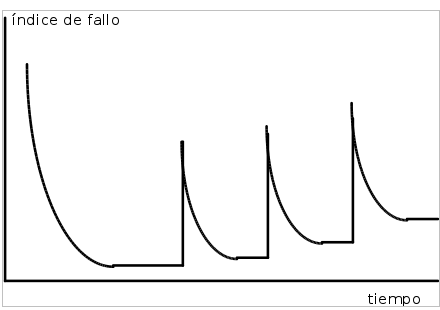
\includegraphics[width=0.4\textwidth]{Resources/fallosSoftwareReales.png}
        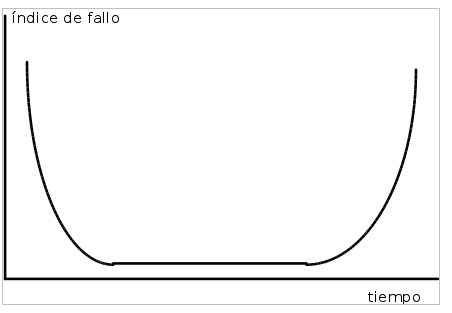
\includegraphics[width=0.4\textwidth]{Resources/fallosHardware.png}
        \caption{Curva de fallos del Software(Izquierda) y del Hardware(Derecha). Obsérvese como en el caso del software el índice de fallos se va acumulando.}
    \end{figure}
    \item \textbf{Baja reutilización de las partes}:
    Por lo general el software se construye a medida como un conjunto, provocando que la reutilización sea baja. Existe una tendencia al alza en la reutilización gracias a:
    \begin{itemize}
        \item La elaboración de librerías y frameworks.
        \item Aplicación de técnicas de programación modular y orientada a objetos de manera estructurada. 
        \item Aplicación de patrones de diseño, que supone en sí misma la reutilización de la estructura ahorrando tiempo en diseño y formación.
    \end{itemize}
\end{enumerate}

\section{Atributos deseables en el software}
\begin{itemize}
    \item \textbf{Mantenibilidad}: Facilidad para realizar cambios.
    \item \textbf{Confiabilidad}: Capacidad para seguir funcionando de manera segura y correcta. 
    \item \textbf{Eficiencia}: Utilización de la mínima cantidad necesaria de recursos.
    \item \textbf{Usabilidad}: Facilidad con la que las personas utilizan el software.
\end{itemize}

\subsection{Aplicaciones del software}
Es difícil clasificarlas y carece de mucho valor hacerlo, \textit{Pressman} lo hace de la siguiente forma, si pregunta características no es difícil deducirlas:
\begin{itemize}
    \item \textbf{Software de sistemas}: Sistemas operativos.
    \item \textbf{Software de aplicación}: Programas independientes que resuelven una necesidad específica.
    \item \textbf{Software científico y de ingeniería}: Simulaciones.
    \item \textbf{Software empotrado}: Corre él solo en un chip.
    \item \textbf{Software de línea de productos}: \textit{Middleware}.
    \item \textbf{Aplicaciones web}.
    \item \textbf{Inteligencia artificial}: \textit{Redes neuronales} (máquinas de estados \textbf{NO}).
\end{itemize}
El objetivo de todo software es desempeñar una determinada función cumpliendo una serie de requisitos.

\section{Software heredado}
Se trata de software \textbf{desarrollado hace décadas} %CORBA 
que además \textbf{ha ido sufriendo cambios} a lo largo del tiempo. Estos dos factores hacen que sea muy difícil de tratar, \uline{y usualmente es crítico para los negocios} (COBOL). \textit{Pressman} aconseja tocarlo lo mínimo posible. 

\section{Principales problemas asociados a la producción del software}
Muchos expertos argumentan que la crisis del software nunca se ha solucionado, y es que esta ingeniería arrastra desde hace tiempo los siguientes \textbf{problemas crónicos}.
\begin{enumerate}
    \item \textbf{Imprecisión en la estimación de costes temporales y monetarios}: Entre las causas podemos citar la falta de recogida de datos de proyectos anteriores y la tradicional falta de experiencia de los gestores (gente que no tiene ni idea de software gestionando proyectos o viceversa).
    \item \textbf{Baja productividad}: El poco énfasis en la recogida de requisitos comúnmente desemboca en tiempo de desarrollo malgastado. Ya bien sea implementando funcionalidad innecesaria o bien por implementarla en un estado de desarrollo avanzado, lo cual es mucho más costoso.
    \item \textbf{Mala calidad}: La falta de realización de pruebas, debida en gran medida a los fallos anteriores, propicia la entrega de software con muchos errores.
    \item \textbf{Insatisfacción del cliente}: Debida a los problemas anteriores no es una tarea agradable contratar software.
\end{enumerate}